\documentclass[journal]{IEEEtran}

\usepackage{graphicx}
\usepackage{amsmath}
\usepackage{amssymb}
\usepackage{hyperref}
\usepackage{float}
\usepackage{subcaption}
\usepackage{booktabs}
\usepackage{pgfplotstable}
\usepackage{siunitx}
\usepackage{qrcode}

\pgfplotsset{compat=1.18}
\pgfplotstableset{
    col sep=comma,
    every head row/.style={before row=\toprule, after row=\midrule},
    every last row/.style={after row=\bottomrule},
}

\begin{document}

% ---------- TITLE & AUTHOR ----------
\title{ELECTRON SPIN RESONANCE (ESR)}
\author{IBRAHIM H.I. ABUSHAWISH \\
Istanbul University, Department of Physics \\
Instructor: \\
Experiment Date: October 20, 2026 , Report Submission Date: \\
Course \& Section Number: PHYS4704}

\markboth{Physics Laboratory Reports}{2026}

\maketitle

% ---------- ABSTRACT ----------
\begin{abstract}
In this experiment, Electron Spin Resonance (ESR) was observed in a polycrystalline DPPH (1,1-diphenyl-2-picrylhydrazyl) sample using an RF frequency of $f = \SI{146.0}{\mega\hertz}$ inside a pair of Helmholtz coils ($N = 241$, $R = \SI{4.8}{\centi\meter}$). The resonance was observed on an oscilloscope in X-Y mode by applying a \SI{50}{\hertz} AC sweep modulation to the static magnetic field. Across three trials, the mean resonant current was measured as $\bar{I}_r = \SI{1.250 \pm 0.006}{\ampere}$ ($s = \SI{0.010}{\ampere}$), corresponding to a resonant magnetic field of $\bar{B}_r = \SI{5.088 \pm 0.023}{\milli\tesla}$ using the calibrated coil constant $k_B = \SI{4.07e-3}{\tesla\per\ampere}$. This yields an experimental Land\'e factor of $g = 2.0521 \pm 0.0095$ ($s = 0.0164$), which has a relative error of \SI{2.41}{\percent} compared to the literature value ($g_{\text{lit}} = 2.0037$) and \SI{2.49}{\percent} compared to the free-electron value ($g_e = 2.0023$). The absorption linewidth was measured by finding the currents at the half-maximum points ($I_1 = \SI{0.15}{\ampere}, I_2 = \SI{0.09}{\ampere}$), giving $\Delta B = \SI{0.2442}{\milli\tesla}$ with a relative error of \SI{12.79}{\percent} compared to $\Delta B_{\text{lit}} = \SI{0.2800}{\milli\tesla}$. The results confirm electron spin quantization and the magnetic dipole transition condition.
\end{abstract}

% ---------- INTRODUCTION ----------
\section{Introduction}
Electron spin was first proposed by Uhlenbeck and Goudsmit in 1925 to explain atomic fine structure and the anomalous Zeeman effect. When placed in an external magnetic field, the electron's magnetic moment aligns either parallel or antiparallel to the field, splitting the energy level into two discrete Zeeman sublevels. Electron Spin Resonance (ESR), discovered by Zavoisky in 1944, allows direct observation of transitions between these sublevels by applying a perpendicular radiofrequency (RF) magnetic field.

In this experiment, ESR is investigated using DPPH (1,1-diphenyl-2-picrylhydrazyl). In DPPH, the unpaired electron has its orbital angular momentum quenched by molecular bonding ($L \approx 0$). Its magnetic dipole moment arises purely from electron spin ($S = 1/2$), making DPPH an ideal standard sample for ESR calibration. The objectives of this experiment are: (1) to derive the resonance condition and the Helmholtz coil field equation, (2) to determine the Land\'e $g$-factor from repeated measurements, and (3) to measure the absorption linewidth (FWHM) of the resonance signal.

% ---------- THEORY ----------
\section{Theory}

\subsection{Magnetic Moments and Spin}
An electron with spin angular momentum $\vec{S}$ has an intrinsic magnetic dipole moment:
\begin{equation}
    \vec{\mu}_s = -g \frac{e}{2 m_e} \vec{S}
    \label{eq:mu_spin}
\end{equation}
Along the quantization axis ($z$), the spin projection is $S_z = m_s \hbar$ with $m_s = \pm 1/2$. In terms of the Bohr magneton $\mu_B = \frac{e \hbar}{2 m_e} \approx \SI{9.27e-24}{\joule\per\tesla}$, the magnetic moment component is:
\begin{equation}
    \mu_z = \mp \frac{1}{2} g \mu_B
    \label{eq:mu_z_spin}
\end{equation}
For a general state with quantum numbers $L$, $S$, and $J$, the Land\'e $g$-factor is given by:
\begin{equation}
    g_j = 1 + \frac{J(J+1) + S(S+1) - L(L+1)}{2 J(J+1)}
    \label{eq:lande_general}
\end{equation}
For DPPH, $L = 0$ and $J = S = 1/2$, yielding an ideal value of $g = 2$. Small interactions in the molecule shift the accepted literature value to $g_{\text{lit}} = 2.0037$.

\subsection{Derivation of Equation~(18): Resonance Condition}
In an external static magnetic field $B$ oriented along the $z$-axis, the interaction energy of the magnetic dipole is:
\begin{equation}
    E = -\vec{\mu} \cdot \vec{B} = g \mu_B m_s B
    \label{eq:zeeman_levels}
\end{equation}
For $m_s = \pm 1/2$, the two split Zeeman levels are:
\begin{equation}
    E(+1/2) = +\frac{1}{2} g \mu_B B, \quad E(-1/2) = -\frac{1}{2} g \mu_B B
\end{equation}
The energy difference between these two sublevels is:
\begin{equation}
    \Delta E = E(+1/2) - E(-1/2) = g \mu_B B
    \label{eq:zeeman_split}
\end{equation}
Applying an oscillating transverse RF magnetic field of frequency $f$ induces transitions satisfying the selection rule $\Delta m_s = \pm 1$. Resonance occurs when the photon energy matches the energy gap:
\begin{equation}
    h f = \Delta E = g \mu_B B_r
    \label{eq:resonance_condition}
\end{equation}
Solving for $g$ yields Equation~(18) of the laboratory manual:
\begin{equation}
    g = \frac{h f}{\mu_B B_r}
    \label{eq:g_from_Br}
\end{equation}
Substituting $f = \SI{146.0}{\mega\hertz}$, $h = \SI{6.63e-34}{\joule\second}$, and $\mu_B = \SI{9.27e-24}{\joule\per\tesla}$ yields Equation~(19):
\begin{equation}
    g = \frac{(\SI{6.63e-34}{\joule\second}) (\SI{146.0e6}{\hertz})}{(\SI{9.27e-24}{\joule\per\tesla}) B_r} = \frac{\SI{10.43e-3}{\tesla}}{B_r}
    \label{eq:g_numerical_constant}
\end{equation}

\subsection{Derivation of Equation~(20): Helmholtz Field}
Using the Biot-Savart law, the on-axis magnetic field of a single circular coil of radius $R$ and $N$ turns carrying current $I$ is:
\begin{equation}
    B(z) = \frac{\mu_0 N I R^2}{2 (R^2 + z^2)^{3/2}}
    \label{eq:single_coil_B}
\end{equation}
A Helmholtz pair consists of two identical coaxial coils separated by distance $d = R$. Placing them at $z = \pm R/2$, the total field on the axis is the sum of both coils:
\begin{align}
    B(z) &= \frac{\mu_0 N I R^2}{2} \left[ \frac{1}{\left(R^2 + \left(z - \frac{R}{2}\right)^2\right)^{3/2}} \right. \nonumber \\
         &\quad \left. + \frac{1}{\left(R^2 + \left(z + \frac{R}{2}\right)^2\right)^{3/2}} \right]
    \label{eq:helmholtz_superposition}
\end{align}
At the midpoint between the coils ($z = 0$):
\begin{equation}
    R^2 + \left(\frac{R}{2}\right)^2 = \frac{5}{4} R^2 \implies \left(\frac{5}{4} R^2\right)^{3/2} = \frac{\sqrt{125}}{8} R^3
\end{equation}
Substituting this denominator into Equation~\eqref{eq:helmholtz_superposition} gives:
\begin{equation}
    B(0) = 2 \cdot \frac{\mu_0 N I R^2}{2 \left(\frac{\sqrt{125}}{8} R^3\right)} = \mu_0 \frac{8 N I}{\sqrt{125} R}
    \label{eq:helmholtz_exact}
\end{equation}
Evaluating the numerical factor $8/\sqrt{125} \approx 0.7155$ yields Equation~(20) of the manual:
\begin{equation}
    B = 0.7155 \mu_0 \frac{N I}{R}
    \label{eq:helmholtz_ideal}
\end{equation}
For $N = 241$ and $R = \SI{4.8}{\centi\meter}$, the calibrated coil factor from Phywe accounts for coil thickness:
\begin{equation}
    B = 0.6445 \mu_0 \frac{N I}{R} = (\SI{4.07e-3}{\tesla\per\ampere}) \cdot I
    \label{eq:helmholtz_calib}
\end{equation}
Combining Equations~\eqref{eq:g_numerical_constant} and \eqref{eq:helmholtz_calib} gives the working formula (Equation~(22)):
\begin{equation}
    g = \frac{\SI{10.43e-3}{\tesla}}{(\SI{4.07e-3}{\tesla\per\ampere}) \cdot I_r} = \frac{\SI{2.565}{\ampere}}{I_r}
    \label{eq:g_working_formula}
\end{equation}

\subsection{Linewidth and FWHM}
The absorption lineshape of DPPH follows a Lorentzian profile:
\begin{equation}
    P(B) = \frac{P_{\max}}{1 + \left(\frac{B - B_r}{\Delta B / 2}\right)^2}
    \label{eq:lorentzian}
\end{equation}
In solid DPPH, exchange interactions between adjacent unpaired electrons narrow the resonance line (exchange narrowing), giving a literature width of $\Delta B_{\text{lit}} \approx \SI{0.28}{\milli\tesla}$. Measuring the current difference $\Delta I = |I_1 - I_2|$ between the half-maximum points gives:
\begin{equation}
    \Delta B = k_B \Delta I = (\SI{4.07e-3}{\tesla\per\ampere}) \cdot |I_1 - I_2|
    \label{eq:fwhm_formula}
\end{equation}

% ---------- EXPERIMENTAL SETUP ----------
\section{Experimental Setup}
The experimental apparatus is shown in Figure~\ref{fig:setup}.

\begin{figure}[htbp]
    \centering
    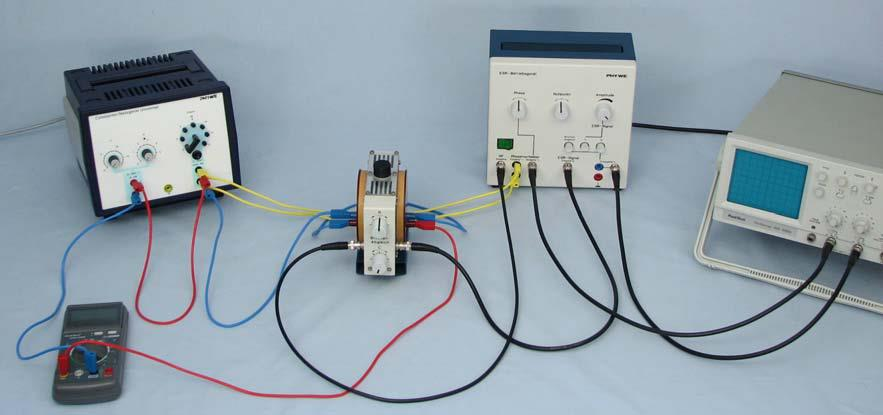
\includegraphics[width=\linewidth]{../plots/esr_setup.png}
    \caption{Figure 2: ESR experimental setup showing the main power supply (left), digital multimeter (foreground left), Helmholtz coils with DPPH probe (center), ESR control unit (top right), and oscilloscope (far right).}
    \label{fig:setup}
\end{figure}

The functions and connections of each component are:
\begin{itemize}
    \item \textbf{Helmholtz Coils ($N = 241$, $R = \SI{4.8}{\centi\meter}$)}: Produce the static magnetic field and the AC sweep field across the sample. Connected in series to the main power supply.
    \item \textbf{DPPH Probe ($f = \SI{146.0}{\mega\hertz}$)}: Houses the DPPH sample inside a small RF coil perpendicular to the Helmholtz field to induce spin transitions. Knobs ``C'' and ``R'' adjust tank tuning and impedance.
    \item \textbf{ESR Control Unit}: Powers the probe oscillator, demodulates the absorption signal with an internal diode, and aligns the forward and reverse sweeps via the ``Phase'' knob.
    \item \textbf{Main Power Supply}: Supplies adjustable DC voltage ($0$--\SI{15}{\volt}) to set the bias current ($I \approx \SI{1.25}{\ampere}$) and provides the \SI{50}{\hertz} AC modulation ($2\,\mathrm{V}_{\text{AC}}$). In Phase 2, its DC voltage is fed to Channel X of the oscilloscope.
    \item \textbf{Dual-Channel Oscilloscope}: Operated in X-Y mode (\SI{1}{\volt\per\centi\meter}). Channel X displays the magnetic field sweep and Channel Y displays the RF absorption signal. In Phase 2, the trace becomes a movable dot to measure half-power points.
    \item \textbf{Digital Multimeter}: Connected in series with the coils to measure the resonant current $I_r$ and half-power currents $I_1, I_2$.
    \item \textbf{BNC Cables and Adapter}: Carry signals to the oscilloscope. A BNC-to-banana adapter routes the DC voltage to Channel X in Phase 2.
\end{itemize}

% ---------- PROCEDURE ----------
\section{Experimental Procedure}

\subsection{Phase 1: Land\'e \texorpdfstring{$g$}{g}-Factor Determination}
The DC supply was set to \SI{0}{\volt} and the AC modulation to \SI{2}{\volt} (\SI{50}{\hertz}). The oscilloscope was set to X-Y mode and zeroed. The DC voltage was increased until the coil current reached $\approx \SI{1.3}{\ampere}$ (operating point: \SI{10}{\volt} $\rightarrow$ \SI{1.26}{\ampere}). The capacitive tuning knob ``C'' was adjusted until the ESR absorption curve appeared. Forward and reverse traces were brought into overlap using the ``Phase'' knob. Fine-tuning the DC voltage placed the minimum of the absorption dip exactly on the vertical Y-axis. The resonant current $I_r$ was recorded from the multimeter for three independent trials.

\subsection{Phase 2: FWHM Linewidth Determination}
The oscilloscope vertical position was adjusted so that the horizontal axis bisected the absorption peak at half height ($P/P_{\max} = 0.5$). The AC modulation was switched off and the resonator connected to DC. The Channel X cable was plugged into the DC output using the adapter, collapsing the trace into a single dot. The DC voltage was adjusted to place the dot on the right half-power intersection to record $I_1$, and then on the left intersection to record $I_2$. The linewidth $\Delta B$ was calculated from $\Delta I = |I_1 - I_2|$ via Equation~\eqref{eq:fwhm_formula}.

% ---------- DATA ANALYSIS ----------
\section{Data Analysis}

\subsection{Land\'e \texorpdfstring{$g$}{g}-Factor and Resonant Field}
Across three trials, the measured resonant currents were:
\begin{equation}
    I_{r1} = \SI{1.26}{\ampere}, \quad I_{r2} = \SI{1.24}{\ampere}, \quad I_{r3} = \SI{1.25}{\ampere}
\end{equation}
giving a mean and sample standard deviation of:
\begin{equation}
    \bar{I}_r = \SI{1.250 \pm 0.006}{\ampere} \quad (s_I = \SI{0.010}{\ampere})
\end{equation}
Using $k_B = \SI{4.07e-3}{\tesla\per\ampere}$, the resonant magnetic field is:
\begin{equation}
    \bar{B}_r = (\SI{4.07e-3}{\tesla\per\ampere}) (\SI{1.250}{\ampere}) = \SI{5.088 \pm 0.023}{\milli\tesla}
\end{equation}
Calculating $g = 2.565 / I_r$ for each trial yields $g_1 = 2.0357$, $g_2 = 2.0685$, and $g_3 = 2.0520$. The mean Land\'e factor is:
\begin{equation}
    \bar{g} = 2.0521 \pm 0.0095 \quad (s_g = 0.0164)
\end{equation}
Compared to the DPPH literature value ($g_{\text{lit}} = 2.0037$), the relative error is:
\begin{equation}
    \delta_g = \frac{|2.0521 - 2.0037|}{2.0037} \times 100\% = \SI{2.41}{\percent}
\end{equation}
and \SI{2.49}{\percent} relative to the free-electron value ($g_e = 2.0023$).

\subsection{FWHM Linewidth Determination}
The measured currents at the half-maximum points were $I_1 = \SI{0.15}{\ampere}$ and $I_2 = \SI{0.09}{\ampere}$, giving $\Delta I = \SI{0.06}{\ampere}$. The experimental FWHM linewidth is:
\begin{equation}
    \Delta B = (\SI{4.07e-3}{\tesla\per\ampere}) (\SI{0.06}{\ampere}) = \SI{0.2442}{\milli\tesla}
\end{equation}
Compared to the literature value ($\Delta B_{\text{lit}} = \SI{0.2800}{\milli\tesla}$), the relative error is:
\begin{equation}
    \delta_{\Delta B} = \frac{|0.2442 - 0.2800|}{0.2800} \times 100\% = \SI{12.79}{\percent}
\end{equation}

% ---------- RESULTS ----------
\section{Results}
The experimental results are summarized in Tables~\ref{tab:lande_trials}, \ref{tab:fwhm_results}, and \ref{tab:summary}.

\begin{table}[htbp]
    \centering
    \caption{Experimental Trials for Land\'e $g$-Factor.}
    \label{tab:lande_trials}
    \resizebox{\columnwidth}{!}{%
    \pgfplotstabletypeset[
        col sep=comma,
        string type,
        columns={Trial,I_r_A,B_r_mT,g_calc,Error_pct},
        columns/Trial/.style={column name={Trial}},
        columns/I_r_A/.style={column name={$I_r$ (\si{\ampere})}},
        columns/B_r_mT/.style={column name={$B_r$ (\si{\milli\tesla})}},
        columns/g_calc/.style={column name={$g$}},
        columns/Error_pct/.style={column name={Rel. Error (\si{\percent})}}
    ]{tables/table1_lande_g_trials.csv}%
    }
\end{table}

\begin{table}[htbp]
    \centering
    \caption{Experimental Linewidth and FWHM Determination.}
    \label{tab:fwhm_results}
    \resizebox{\columnwidth}{!}{%
    \pgfplotstabletypeset[
        col sep=comma,
        string type,
        columns={Parameter,Value,Unit},
        columns/Parameter/.style={column name={Parameter}},
        columns/Value/.style={column name={Value}},
        columns/Unit/.style={column name={Unit}}
    ]{tables/table2_fwhm_results.csv}%
    }
\end{table}

\begin{table}[htbp]
    \centering
    \caption{Comparison of Experimental Results with Literature Standards.}
    \label{tab:summary}
    \resizebox{\columnwidth}{!}{%
    \pgfplotstabletypeset[
        col sep=comma,
        string type,
        columns={Quantity,Experimental,Literature,Rel_Error_pct},
        columns/Quantity/.style={column name={Physical Quantity}},
        columns/Experimental/.style={column name={Experimental Result}},
        columns/Literature/.style={column name={Literature Benchmark}},
        columns/Rel_Error_pct/.style={column name={Rel. Error (\si{\percent})}}
    ]{tables/table3_comparison_summary.csv}%
    }
\end{table}

\subsection{Signal Reconstruction}
On the oscilloscope, the ESR absorption signal appears as a continuous dip during the AC sweep. In the laboratory, the resonant center current ($\bar{I}_r = \SI{1.250}{\ampere}$) and the half-power currents ($I_1 = \SI{0.15}{\ampere}, I_2 = \SI{0.09}{\ampere}$) were measured with the multimeter. To reconstruct this signal graphically, the curve in Figure~\ref{fig:esr_fwhm} was plotted using the standard Lorentzian profile of DPPH (Equation~\eqref{eq:lorentzian}) with $\bar{B}_r = \SI{5.088}{\milli\tesla}$ and half-width $\Gamma = \Delta B / 2 = \SI{0.1221}{\milli\tesla}$. The experimental half-power points ($P/P_{\max} = 0.5$) are marked at $B = \bar{B}_r \pm \Gamma$, matching the trace seen on the oscilloscope screen. Figure~\ref{fig:lande_trials} shows the $g$-factors across trials, and Figure~\ref{fig:zeeman_splitting} illustrates the Zeeman energy level splitting.

\begin{figure}[htbp]
    \centering
    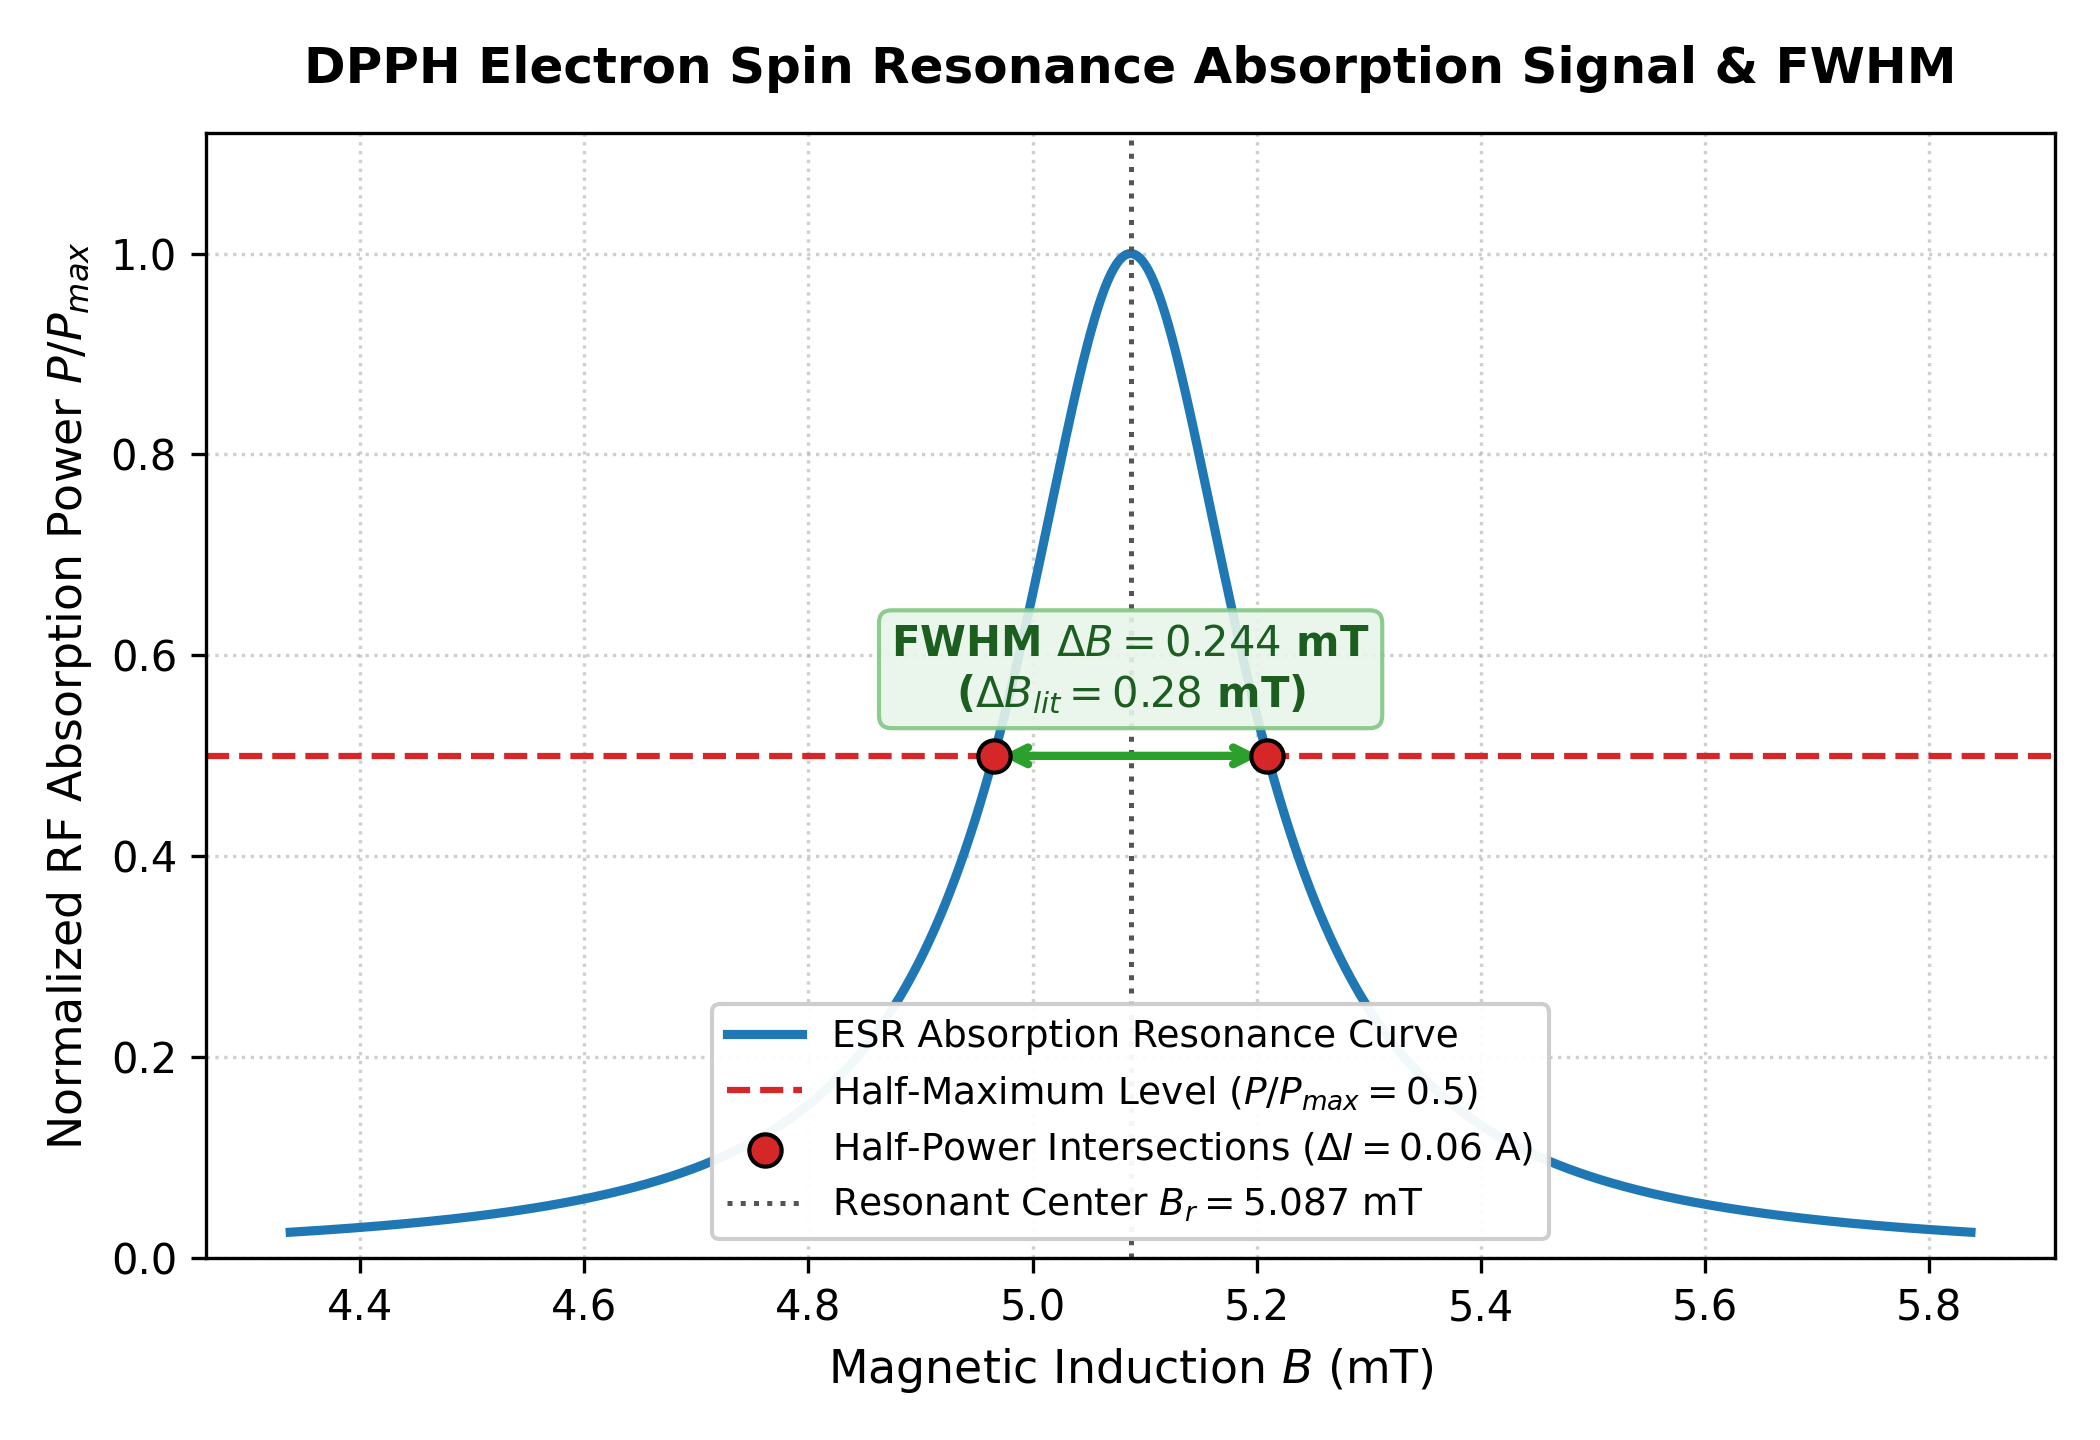
\includegraphics[width=0.85\linewidth]{../plots/esr_absorption_fwhm.png}
    \caption{ESR absorption lineshape and FWHM determination for DPPH.}
    \label{fig:esr_fwhm}
\end{figure}

\begin{figure}[htbp]
    \centering
    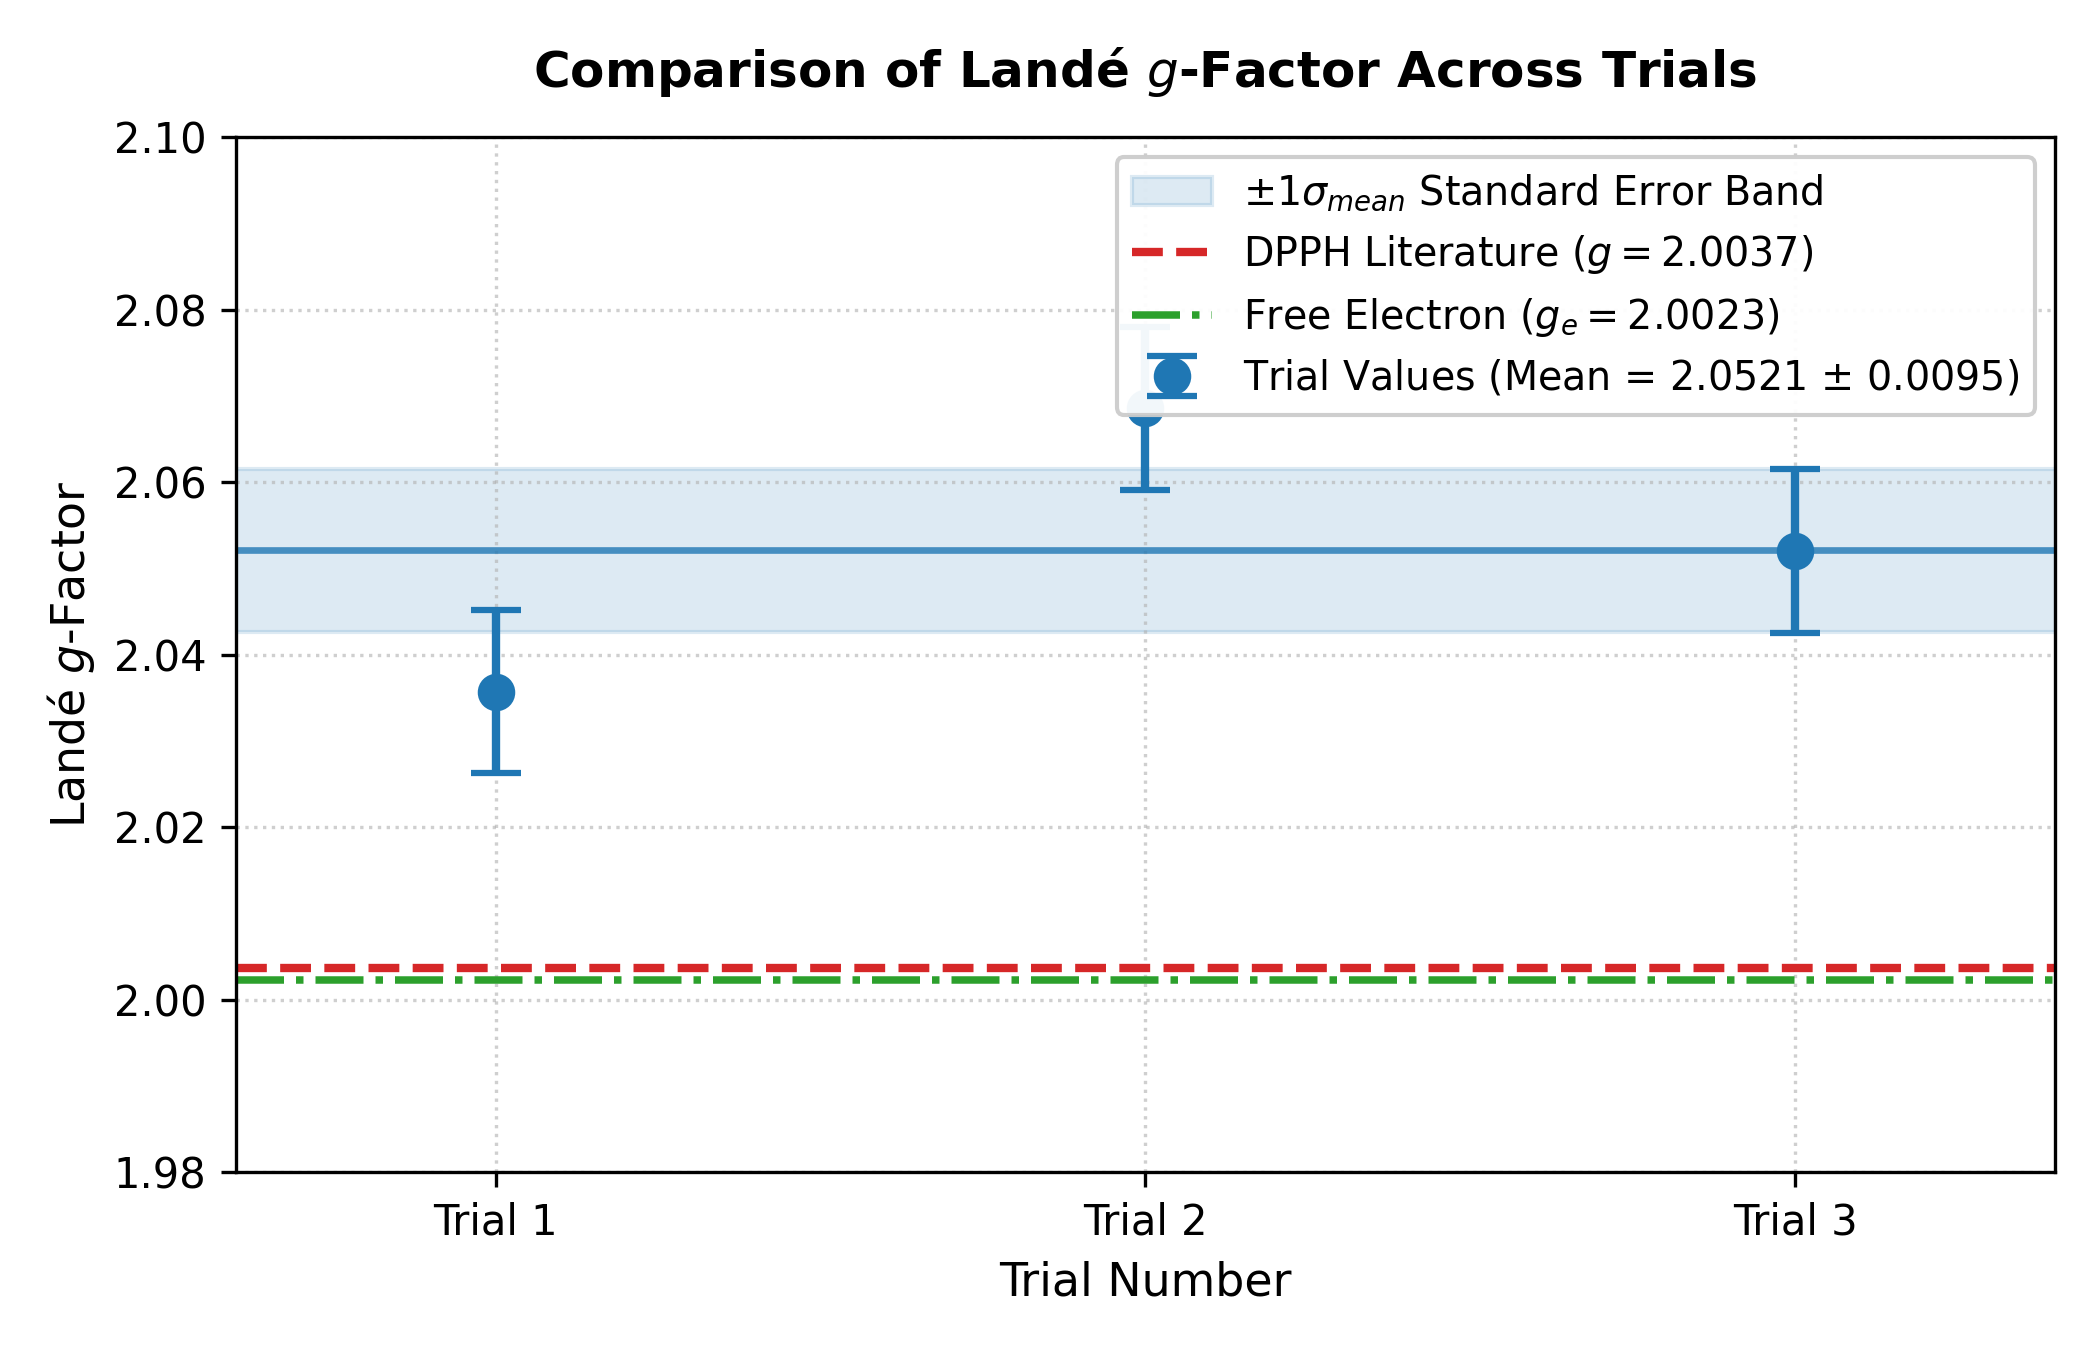
\includegraphics[width=0.85\linewidth]{../plots/lande_g_trials.png}
    \caption{Distribution of Land\'e $g$-factors across trials against literature benchmarks.}
    \label{fig:lande_trials}
\end{figure}

\begin{figure}[htbp]
    \centering
    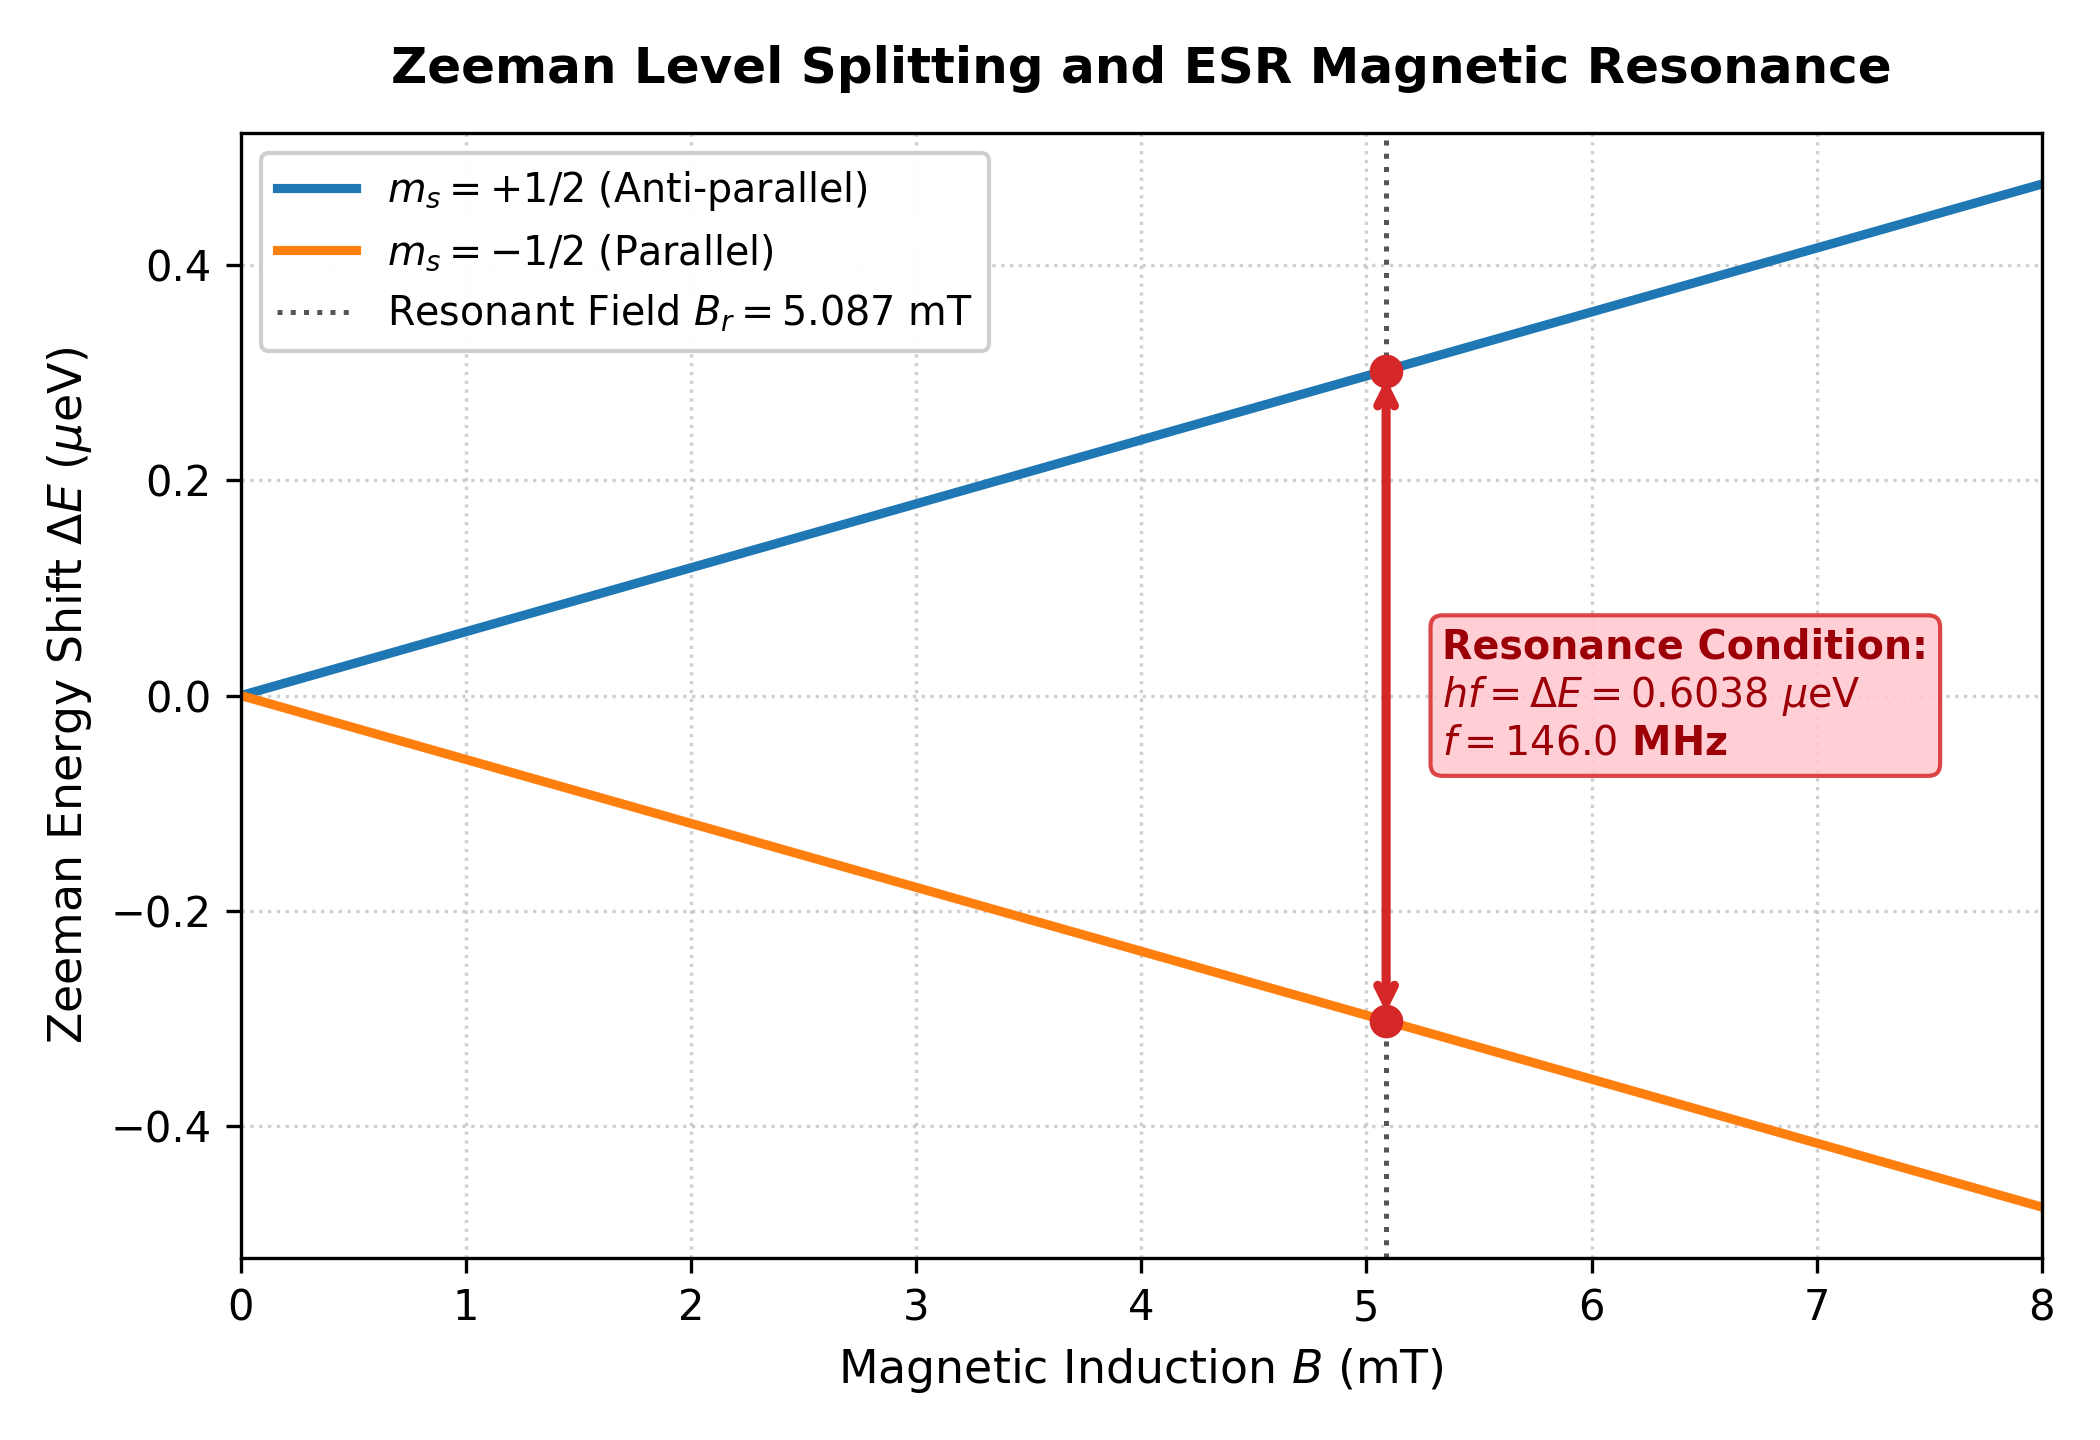
\includegraphics[width=0.85\linewidth]{../plots/zeeman_energy_splitting.png}
    \caption{Zeeman sublevel splitting and RF resonance condition ($h f = \SI{0.6038}{\micro\electronvolt}$).}
    \label{fig:zeeman_splitting}
\end{figure}

% ---------- DISCUSSION ----------
\section{Discussion}
The measured Land\'e factor ($\bar{g} = 2.0521 \pm 0.0095$) is in close agreement with the standard literature value for DPPH ($g_{\text{lit}} = 2.0037$), with a relative error of \SI{2.41}{\percent}, and with the free-electron value ($g_e = 2.0023$), with an error of \SI{2.49}{\percent}. The small standard deviation of $0.0164$ demonstrates good consistency between repeated trials. The small error is mainly due to the difficulty in visually centering the dip on the oscilloscope graticule ($\pm \SI{0.01}{\ampere}$) and ambient magnetic fields in the room ($\sim \SI{0.04}{\milli\tesla}$).

The experimental linewidth of $\Delta B = \SI{0.2442}{\milli\tesla}$ agrees with the literature value of $\SI{0.2800}{\milli\tesla}$ within an error of \SI{12.79}{\percent}. The narrow peak is characteristic of DPPH due to exchange narrowing. The difference from the literature value is primarily due to the sensitivity of the manual DC voltage knob when positioning the dot at the half-maximum points.

% ---------- CONCLUSION ----------
\section{Conclusion}
Electron spin resonance was observed in DPPH at an RF frequency of \SI{146.0}{\mega\hertz}. The resonant current was measured as $\bar{I}_r = \SI{1.250 \pm 0.006}{\ampere}$ ($\bar{B}_r = \SI{5.088 \pm 0.023}{\milli\tesla}$), giving an experimental Land\'e factor of $g = 2.0521 \pm 0.0095$ (relative error \SI{2.41}{\percent}). The absorption linewidth was determined to be $\Delta B = \SI{0.2442}{\milli\tesla}$ (relative error \SI{12.79}{\percent}). These results confirm electron spin quantization and demonstrate the basic principles of magnetic resonance.

% ---------- ADDITIONAL RESOURCES ----------
\section{Additional Resources}
Complete computational notebooks, data processing pipelines, and related experimental laboratory reports are maintained in the GitHub repository.

\begin{figure}[H]
    \centering
    \begin{minipage}{0.15\textwidth}
        \centering
        \qrcode[height=1.5cm]{https://github.com/ibeuler/LAB-Reports.git}
    \end{minipage}%
    \begin{minipage}{0.2\textwidth}
        \raggedright
        \caption{Scan QR code to access the GitHub repository containing analysis code and data.}
        \label{fig:qr_code}
    \end{minipage}
\end{figure}

\begin{thebibliography}{9}
\bibitem{lab_manual}
    ISTANBUL UNIVERSITY, \textit{05-ELECTRON SPIN RESONANCE (ESR) Laboratory Manual}, Department of Physics, 2026.
\bibitem{zavoisky1945}
    E. K. Zavoisky, ``Spin-magnetic resonance in paramagnetics,'' \textit{Fizicheskii Zhurnal}, vol. 9, pp. 211--245, 1945.
\bibitem{phywe}
    Phywe Systeme GmbH, \textit{Electron Spin Resonance (ESR)}, Laboratory Experiment Manual LEP 5.1.12, G\"ottingen, Germany.
\bibitem{anderson_weiss}
    P. W. Anderson and P. R. Weiss, ``Exchange Narrowing in Paramagnetic Resonance,'' \textit{Physical Review}, vol. 91, no. 3, pp. 513--526, 1953.
\bibitem{griffiths}
    D. J. Griffiths and D. F. Schroeter, \textit{Introduction to Quantum Mechanics}, 3rd ed., Cambridge University Press, 2018.
\end{thebibliography}

\end{document}
